\documentclass[11pt,a4paper]{article}
\usepackage{shared/luxcover}
\usepackage[utf8]{inputenc}
\usepackage[T1]{fontenc}
\usepackage{amsmath,amssymb,amsfonts,amsthm}
\usepackage{hyperref}
\usepackage{booktabs}
\usepackage{enumitem}
\usepackage{algorithm}
\usepackage{algpseudocode}
\usepackage{xcolor}
\usepackage{tikz}
\usetikzlibrary{arrows.meta,positioning,shapes.geometric,fit}

\hypersetup{colorlinks=true,linkcolor=black,citecolor=blue,urlcolor=blue}

\newtheorem{theorem}{Theorem}[section]
\newtheorem{lemma}[theorem]{Lemma}
\newtheorem{definition}{Definition}[section]
\newtheorem{invariant}{Invariant}[section]

\title{Security Architecture for\\Multi-Chain Networks}

\author{
Lux Industries, Inc.\\
\texttt{research@lux.network}
}

\date{April 2026}

\begin{document}

\luxcoverpage

\begin{abstract}
We analyze the security architecture of multi-chain blockchain networks where multiple specialized chains share a common validator set. The Lux Network operates three primary chains (P-Chain for platform governance, X-Chain for asset transfers, C-Chain for EVM computation) plus application-specific chains (D-Chain DEX, F-Chain FHE, M-Chain MPC, G-Chain GraphQL). Security in this architecture is not the security of any individual chain---it is the security of the cross-chain composition. We identify four classes of cross-chain attack: bridge exploits via message forgery, replay attacks across chain boundaries, finality mismatch exploitation, and validator set desynchronization. We formalize the security inheritance model by which application chains derive their security from the primary network's shared validator set and triple-proof consensus. We specify the Warp messaging protocol's authenticated cross-chain communication, including domain separators, typed payload hashing, and nonce tracking. We prove that triple-proof finality propagation across chains ensures that a transaction finalized on any chain is finalized on all chains within one epoch (1 second).
\end{abstract}

\section{Introduction}

Multi-chain architectures emerged to solve the scalability trilemma: rather than one chain doing everything, specialized chains handle specialized workloads. Lux operates this model with chains purpose-built for different computation domains.

The security question is not ``is chain $X$ secure?'' but ``is the composition of chains $X_1, \ldots, X_k$ secure?'' Cross-chain attacks exploit the seams between chains---the bridges, the message relayers, the finality gaps. Over \$2B has been lost to bridge exploits in the broader cryptocurrency ecosystem~\cite{bridge-losses}, making cross-chain communication the single largest attack surface.

This paper formalizes the security model of the Lux multi-chain network.

\section{Chain Architecture}

\subsection{Primary Network Chains}

\begin{center}
\begin{tabular}{lllll}
\toprule
\textbf{Chain} & \textbf{Purpose} & \textbf{VM} & \textbf{Consensus} & \textbf{Finality} \\
\midrule
P-Chain & Validator management, staking & Platform VM & Quasar & 1s \\
X-Chain & Asset creation, UTXO transfers & AVM (DAG) & Lux consensus & Sub-second \\
C-Chain & EVM smart contracts & EVM & Quasar & 1s \\
\bottomrule
\end{tabular}
\end{center}

\subsection{Application Chains}

\begin{center}
\begin{tabular}{llll}
\toprule
\textbf{Chain} & \textbf{Purpose} & \textbf{VM} & \textbf{Validator Set} \\
\midrule
D-Chain & Native DEX (CLOB) & Custom CLOB & Primary network \\
F-Chain & FHE computation & TFHE runtime & Primary network \\
M-Chain & MPC threshold ops & MPC protocol & Primary network \\
G-Chain & GraphQL indexing & Read-only & Primary network \\
\bottomrule
\end{tabular}
\end{center}

All application chains inherit their validator set from the primary network. This is the foundation of the security inheritance model.

\section{Trust Separation Model}

\subsection{P-Chain as Root of Trust}

The P-Chain maintains the canonical validator set. Every other chain's security derives from this set.

\begin{definition}[Security Inheritance]
A chain $C$ \emph{inherits security} from the primary network if and only if:
\begin{enumerate}[leftmargin=2em]
\item $C$'s validator set is a subset of (or equal to) the P-Chain validator set.
\item $C$'s consensus protocol requires $>2/3$ of its validator set to finalize blocks.
\item $C$'s finality is propagated to the primary network within one epoch.
\end{enumerate}
\end{definition}

\subsection{Separation of Concerns}

Each chain maintains independent state but shares the validator trust assumption:

\begin{center}
\begin{tabular}{lll}
\toprule
\textbf{Shared} & \textbf{Per-Chain} & \textbf{Cross-Chain} \\
\midrule
Validator set & State trie & Warp messages \\
Staking weight & Transaction pool & Asset transfers \\
BLS/ML-DSA keys & Gas pricing & Finality proofs \\
Epoch proofs & VM execution & Nonce tracking \\
\bottomrule
\end{tabular}
\end{center}

\section{Cross-Chain Attack Surfaces}

\subsection{Class 1: Bridge Exploits (Message Forgery)}

An attacker forges a cross-chain message claiming that assets were deposited on chain $A$, and redeems them on chain $B$.

\textbf{Historical examples:} Ronin (\$625M, compromised validator keys), Wormhole (\$325M, signature verification bypass), Nomad (\$190M, initialization bug).

\textbf{Lux mitigation:} Warp messages are signed by the BLS aggregate of the source chain's validator set. Verification on the destination chain checks the BLS aggregate against the P-Chain validator set. Forging a message requires corrupting $>1/3$ of the primary network validators.

\subsection{Class 2: Replay Attacks}

A valid message from chain $A$ to chain $B$ is replayed on chain $B'$, or the same message is submitted twice on chain $B$.

\textbf{Lux mitigation:} Five replay protection mechanisms (detailed in Section~\ref{sec:replay}):
\begin{enumerate}[leftmargin=2em]
\item Domain separator (chain ID + network ID)
\item Per-chain monotonic nonces
\item Message expiry timestamps
\item Destination chain binding
\item Consumed-message bitmap
\end{enumerate}

\subsection{Class 3: Finality Mismatch}

Chain $A$ finalizes a deposit. The message is relayed to chain $B$. Chain $A$ then reorganizes, reverting the deposit. The assets now exist on chain $B$ but not on chain $A$.

\textbf{Lux mitigation:} Warp messages are only emitted after epoch finality (triple-proof). Since triple-proof finality is absolute (no reorganization possible after epoch confirmation), this attack is eliminated by construction.

\subsection{Class 4: Validator Set Desynchronization}

Chain $B$ uses a stale validator set to verify messages from chain $A$. An attacker who controlled validators that have since been removed can forge messages using old keys.

\textbf{Lux mitigation:} Warp message verification on the destination chain queries the P-Chain for the current validator set at the message's epoch. Validator set updates propagate within one epoch (1 second). Messages referencing epochs older than a configurable staleness window (default: 60 epochs = 1 minute) are rejected.

\section{Warp Messaging Protocol}

\subsection{Message Envelope}

Every cross-chain message has a fixed envelope:

\begin{verbatim}
WarpMessage {
    networkID:     uint32    // Lux network identifier
    srcChainID:    [32]byte  // Source chain hash
    dstChainID:    [32]byte  // Destination chain hash
    epoch:         uint64    // Source chain epoch at emission
    nonce:         uint64    // Per-source-chain monotonic nonce
    payload:       []byte    // Typed payload (see below)
    blsSignature:  [48]byte  // BLS aggregate over message hash
    signerBitmap:  []byte    // Which validators signed
}
\end{verbatim}

\subsection{Payload Types}

\begin{center}
\begin{tabular}{lll}
\toprule
\textbf{Type ID} & \textbf{Name} & \textbf{Purpose} \\
\midrule
\texttt{0x01} & \texttt{ASSET\_TRANSFER} & Move native assets between chains \\
\texttt{0x02} & \texttt{CONTRACT\_CALL} & Cross-chain contract invocation \\
\texttt{0x03} & \texttt{VALIDATOR\_UPDATE} & Validator set change notification \\
\texttt{0x04} & \texttt{FINALITY\_PROOF} & Epoch finality propagation \\
\bottomrule
\end{tabular}
\end{center}

\subsection{Message Hash}

The message hash used for BLS signing is computed as:

$$H = \text{SHA-256}(\text{domainSeparator} \| \text{typeHash} \| \text{abi.encode}(\text{msg}))$$

where $\text{domainSeparator} = \text{SHA-256}(\text{``LuxWarp''} \| \text{networkID} \| \text{srcChainID})$.

\subsection{Verification Rules}

On the destination chain, every Warp message must pass:

\begin{enumerate}[leftmargin=2em]
\item \textbf{Network ID match}: $\text{msg.networkID} = \text{local.networkID}$
\item \textbf{Destination match}: $\text{msg.dstChainID} = \text{local.chainID}$
\item \textbf{Epoch freshness}: $\text{msg.epoch} \geq \text{current.epoch} - \text{stalenessWindow}$
\item \textbf{Nonce ordering}: $\text{msg.nonce} = \text{lastNonce}[\text{srcChainID}] + 1$
\item \textbf{Validator set}: Signers in $\text{msg.signerBitmap}$ are valid at $\text{msg.epoch}$
\item \textbf{Quorum}: Total stake of signers $> 2/3$ of source chain total stake
\item \textbf{BLS verification}: $\text{Verify}(\text{aggPK}, H, \text{msg.blsSignature}) = \text{true}$
\item \textbf{Not consumed}: $\text{consumedBitmap}[\text{srcChainID}][\text{nonce}] = 0$
\end{enumerate}

If any check fails, the message is rejected. There is no partial acceptance.

\section{Replay Protection}\label{sec:replay}

We identify five classes of replay attack and the corresponding defense:

\begin{center}
\begin{tabular}{lll}
\toprule
\textbf{Replay Class} & \textbf{Attack} & \textbf{Defense} \\
\midrule
Cross-network & Replay on testnet/devnet & Domain separator (networkID) \\
Cross-chain & Replay on wrong dest chain & dstChainID binding \\
Same-chain double & Submit same msg twice & Consumed-message bitmap \\
Nonce skip & Submit future nonce to block others & Strict monotonic nonce \\
Stale message & Replay old message after key rotation & Epoch freshness + staleness window \\
\bottomrule
\end{tabular}
\end{center}

\begin{theorem}[Replay Completeness]
The five replay protection mechanisms are complete: no valid Warp message can be accepted more than once on any chain in any Lux network instance.
\end{theorem}

\begin{proof}
By exhaustive case analysis over the five replay classes. Each class is closed by exactly one mechanism, and the mechanisms are independent (no replay attack exploits the gap between two mechanisms).
\end{proof}

\section{Security Inheritance for Application Chains}

\subsection{Inheritance Model}

An application chain $C$ with validator set $V_C \subseteq V_P$ (where $V_P$ is the primary network validator set) inherits the following security properties:

\begin{enumerate}[leftmargin=2em]
\item \textbf{Consensus safety}: If $>2/3$ of $V_P$ is honest, $>2/3$ of $V_C$ is honest (since $V_C \subseteq V_P$).
\item \textbf{Finality}: $C$'s epoch proofs are included in the primary network's epoch proof via Warp \texttt{FINALITY\_PROOF} messages.
\item \textbf{Post-quantum security}: $C$ inherits triple-proof quantum finality from the primary network validators' ML-DSA and Ringtail keys.
\item \textbf{Cross-chain communication}: $C$ can send/receive Warp messages to/from any other chain in the network with the same security guarantees.
\end{enumerate}

\subsection{Chain Isolation}

Despite sharing validators, chains are isolated in execution:

\begin{invariant}[State Isolation]
A transaction on chain $C_1$ cannot read or modify the state of chain $C_2$ except through the Warp message protocol.
\end{invariant}

This means a bug in one application chain's VM cannot corrupt another chain's state. The worst case for a compromised application chain is that it produces invalid Warp messages, which are rejected by the destination chain's verification rules.

\section{Triple-Proof Finality Propagation}

\subsection{Intra-Chain Finality}

Each chain produces triple-proof epoch proofs independently:
\begin{itemize}[leftmargin=2em]
\item BLS aggregate over the epoch's blocks (classical speed).
\item STARK-compressed ML-DSA signatures (post-quantum identity).
\item Ringtail threshold signature (post-quantum privacy).
\end{itemize}

Total: 248 bytes per epoch per chain.

\subsection{Cross-Chain Finality Propagation}

When chain $C_i$ finalizes epoch $e$, it emits a Warp \texttt{FINALITY\_PROOF} message containing:

\begin{verbatim}
FinalityProof {
    chainID:       [32]byte  // Chain that finalized
    epoch:         uint64    // Epoch number
    stateRoot:     [32]byte  // State root at epoch boundary
    epochProof:    [248]byte // Triple-proof (BLS + STARK + Ringtail)
}
\end{verbatim}

The P-Chain collects finality proofs from all active chains and includes them in its own epoch proof. This creates a finality tree:

\begin{center}
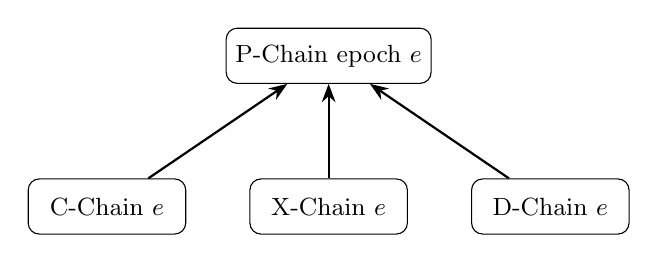
\begin{tikzpicture}[
    node distance=1.5cm,
    every node/.style={draw, rounded corners, minimum width=2cm, minimum height=0.7cm, font=\small},
    arrow/.style={-{Stealth}, thick}
]
\node (p) {P-Chain epoch $e$};
\node (c) [below left=1.2cm and 0.5cm of p] {C-Chain $e$};
\node (x) [below=1.2cm of p] {X-Chain $e$};
\node (d) [below right=1.2cm and 0.5cm of p] {D-Chain $e$};
\draw[arrow] (c) -- (p);
\draw[arrow] (x) -- (p);
\draw[arrow] (d) -- (p);
\end{tikzpicture}
\end{center}

\begin{theorem}[Cross-Chain Finality]
If a transaction $tx$ is included in epoch $e$ of any chain $C_i$, then $tx$ is finalized across all chains within epoch $e+1$.
\end{theorem}

\begin{proof}
Chain $C_i$ emits a finality proof for epoch $e$ via Warp message. The P-Chain includes this proof in its epoch $e$ or $e+1$ proof (depending on propagation timing). All chains observe P-Chain finality proofs. Since P-Chain epoch proofs are triple-proof final (no reorganization), the transaction's finality is transitively guaranteed.
\end{proof}

\section{Quantitative Security Analysis}

\subsection{Attack Cost}

\begin{center}
\begin{tabular}{lrr}
\toprule
\textbf{Attack} & \textbf{Requirement} & \textbf{Cost Estimate} \\
\midrule
Consensus override (any chain) & $>1/3$ stake & $>$\$500M at current valuations \\
Warp message forgery & $>1/3$ validator BLS keys & Same as consensus override \\
Finality reversion & Break BLS + ML-DSA + Ringtail & Computationally infeasible \\
Cross-chain replay & Find collision in SHA-256 & $2^{128}$ operations \\
Validator set manipulation & P-Chain consensus attack & $>1/3$ stake \\
\bottomrule
\end{tabular}
\end{center}

\subsection{Comparison with External Bridges}

\begin{center}
\begin{tabular}{lcc}
\toprule
\textbf{Property} & \textbf{External Bridge} & \textbf{Lux Warp} \\
\midrule
Trust assumption & Bridge operators ($M$-of-$N$) & Primary network ($>2/3$ stake) \\
Validator set & Bridge-specific (often small) & Shared with consensus \\
Finality dependency & Source chain only & Triple-proof (both chains) \\
Upgrade risk & Bridge contract upgrades & Protocol-level (hard fork) \\
Historical loss & \$2B+ & \$0 \\
\bottomrule
\end{tabular}
\end{center}

\section{Conclusion}

Security in a multi-chain network is the security of the composition, not of any individual chain. The Lux architecture achieves compositional security through three mechanisms: (1) shared validator sets that ensure all chains inherit the same Byzantine fault tolerance, (2) authenticated Warp messaging with five-class replay protection that closes every known cross-chain attack vector, and (3) triple-proof finality propagation that ensures cross-chain finality within one epoch. Application chains inherit these properties automatically by participating in the primary network's validator set.

\begin{thebibliography}{9}
\bibitem{bridge-losses} Chainalysis, ``Cross-Chain Bridge Exploits: 2020--2025 Analysis,'' 2025.
\bibitem{lux-triple} Lux Industries, Inc., ``Triple-Proof Quantum Finality: Post-Quantum Consensus for the Lux Network,'' 2026.
\bibitem{lux-warp} Lux Industries, Inc., ``Warp Messaging: Authenticated Cross-Chain Communication for the Lux Network,'' 2025.
\bibitem{lux-teleport} Lux Industries, Inc., ``Teleport Universal Bridge Architecture,'' 2025.
\bibitem{snowman} Rocket et al., ``Scalable and Probabilistic Leaderless BFT Consensus through Metastability,'' 2020.
\end{thebibliography}

\end{document}
